% ============================================================
% Lecture 2: scaling limits of neural networks
% ============================================================
\chapter{Scaling Limits of Neural Networks}
\label{ch:lecture2}

\begin{keyideas}
\begin{itemize}
    \item Large networks are controlled by a few \emph{dimensionless ratios},
    not by the raw sizes. A scaling limit is specified by the path to
    infinity together with how the hyperparameters scale.
    \item \textbf{Deep linear network:}
    $\log\bigl(\|z^{(L)}\|/\|x\|\bigr)\to\mathcal N(-\xi/2,\xi/2)$ with
    effective depth $\xi=L/N$; the width-first and depth-first limits differ.
    \item \textbf{ResNet:} $s_L\sim L^{-1/2}$ is critical for iid layers and
    gives a Neural SDE; $s_L\sim L^{-1}$ requires weights that vary smoothly
    across depth and gives a Neural ODE; correlated weights with Hurst
    exponent $H$ interpolate via $s_L\sim L^{-H}$.
    \item \textbf{Ridge regression:} at $\gamma=d/n$ the Marchenko--Pastur law
    gives the exact asymptotic risk, minimized at
    $\lambda_*=\gamma/\mathrm{SNR}$.
\end{itemize}
\end{keyideas}

\section{Basic setup}

\textbf{Definition (MLP).}
For an input
\[
x\in\mathbb{R}^{N_0},
\]
a multilayer perceptron is defined recursively by
\begin{align}
    z^{(1)}(x)
    &=
    W^{(1)}x+b^{(1)}
    \in\mathbb{R}^{N_1},
    \\
    z^{(\ell+1)}(x)
    &=
    W^{(\ell+1)}
    \phi\!\left(z^{(\ell)}(x)\right)
    +
    b^{(\ell+1)},
    \qquad
    \ell=1,\dots,L-1.
\end{align}
Here \(N_\ell\) is the width of layer \(\ell\), while \(L\) is the
depth of the network.  In the simplest constant-width setting,
\[
N_1=\cdots=N_L=N.
\]

\medskip

\textbf{Definition (ResNet).}
A residual network takes the form
\begin{equation}
    z^{(\ell+1)}
    =
    z^{(\ell)}
    +
    s_L F^{(\ell)}\!\left(z^{(\ell)}\right),
\end{equation}
where, for example,
\begin{equation}
    F^{(\ell)}(z)
    =
    W_2^{(\ell)}
    \phi\!\left(
        W_1^{(\ell)}z+b_1^{(\ell)}
    \right)
    +
    b_2^{(\ell)}.
\end{equation}
The factor \(s_L\) controls how the residual branch must scale as
the depth \(L\) increases.

\section{The scaling question}

A central question is:

\begin{quote}
\emph{What limiting dynamics arise when the model size, data size,
and training time all become large?}
\end{quote}

There are many possible large parameters.

\paragraph{Model scales.}
\begin{itemize}
    \item depth \(L\),
    \item width \(N\),
    \item number of attention heads \(H\),
    \item embedding dimension, number of parameters, etc.
\end{itemize}

\paragraph{Data and optimization scales.}
\begin{itemize}
    \item number of data points \(n\),
    \item batch size \(B\),
    \item number of optimization steps \(T\).
\end{itemize}

It is not enough to simply say that all of these quantities go to
infinity.  One must specify the \emph{path} to infinity and how the
hyperparameters scale:
\begin{equation}
    \mathcal{H}
    =
    \left\{
        \eta,\,
        \sigma,\,
        B,\,
        \lambda,\ldots
    \right\}
    =
    \mathcal{H}(L,N,n,T,\ldots).
\end{equation}

\paragraph{Motivations.}
\begin{enumerate}
    \item Identify a small number of macroscopic variables that
    describe learning, analogous to thermodynamic variables in
    statistical physics.  Examples include activation norms,
    feature covariances, kernel spectra, and training loss.

    \item Identify parameterizations for which scaling is predictable:
    when the model becomes larger, one would like quantities such as
    the optimal learning rate or initialization scale to remain
    controlled.  This is the idea behind \emph{hyperparameter transfer}.
\end{enumerate}

We first study three simple examples:
\begin{enumerate}
    \item depth \(L\) versus width \(N\) in a fully connected network;
    \item the large-depth limit of a ResNet;
    \item parameter dimension \(d\) versus number of data points \(n\).
\end{enumerate}


% ============================================================
\section{Depth versus width: deep linear networks}
% ============================================================

We first remove all nonlinear complications and take
\[
\phi(z)=z,
\qquad
b^{(\ell)}=0.
\]
Then
\begin{equation}
    z^{(L)}(x)
    =
    W^{(L)}W^{(L-1)}\cdots W^{(1)}x.
\end{equation}

Assume all hidden layers have width \(N\), and initialize
\begin{equation}
    W_{ij}^{(\ell)}
    \overset{\mathrm{iid}}{\sim}
    \mathcal{N}\!\left(0,\frac{1}{N}\right).
\end{equation}
The \(1/N\) variance scaling is the natural random-matrix scaling:
for a fixed vector \(v\),
\begin{equation}
    \mathbb{E}\left[
        \|W^{(\ell)}v\|_2^2
        \mid v
    \right]
    =
    \|v\|_2^2.
\end{equation}

More precisely, rotational invariance gives
\begin{equation}
    \frac{
        \left\|W^{(\ell)}v\right\|_2^2
    }{
        \|v\|_2^2
    }
    \overset{d}{=}
    \frac{1}{N}\chi_N^2.
\end{equation}
Since different layers are independent,
\begin{equation}
    \frac{\|z^{(L)}(x)\|_2}{\|x\|_2}
    \overset{d}{=}
    \prod_{\ell=1}^L
    \sqrt{\frac{\chi_{N,\ell}^2}{N}},
\end{equation}
where the \(\chi_{N,\ell}^2\)'s are independent.

Taking the logarithm turns the product into a sum:
\begin{equation}
    \log
    \frac{\|z^{(L)}(x)\|_2}{\|x\|_2}
    =
    \frac{1}{2}
    \sum_{\ell=1}^L
    \log\left(
        \frac{\chi_{N,\ell}^2}{N}
    \right).
\end{equation}

For large \(N\),
\begin{align}
    \mathbb{E}
    \left[
        \log\left(
            \frac{\chi_N^2}{N}
        \right)
    \right]
    &=
    -\frac{1}{N}
    +
    O(N^{-2}),
    \\
    \operatorname{Var}
    \left[
        \log\left(
            \frac{\chi_N^2}{N}
        \right)
    \right]
    &=
    \frac{2}{N}
    +
    O(N^{-2}).
\end{align}
Therefore,
\begin{equation}
    \log
    \frac{\|z^{(L)}(x)\|_2}{\|x\|_2}
    \approx
    \mathcal{N}\!\left(
        -\frac{L}{2N},
        \frac{L}{2N}
    \right).
\end{equation}

This immediately identifies the natural dimensionless parameter
\begin{equation}
    \boxed{
        \xi=\frac{L}{N}
    }
\end{equation}
which acts as an \emph{effective depth}.

If
\[
L,N\rightarrow\infty,
\qquad
\frac{L}{N}\rightarrow\xi,
\]
then
\begin{equation}
    \boxed{
    \log
    \frac{\|z^{(L)}(x)\|_2}{\|x\|_2}
    \Longrightarrow
    \mathcal{N}
    \left(
        -\frac{\xi}{2},
        \frac{\xi}{2}
    \right).
    }
\end{equation}
Thus the norm becomes approximately log-normal.

\paragraph{Important subtlety.}
Although
\begin{equation}
    \mathbb{E}\|z^{(L)}(x)\|_2^2
    =
    \|x\|_2^2
\end{equation}
for every \(L\), the \emph{typical} norm decreases:
\[
\mathbb{E}
\left[
    \log
    \frac{\|z^{(L)}(x)\|_2}{\|x\|_2}
\right]
<0.
\]
The conserved second moment is maintained by increasingly rare
realizations with large norms.  This is the distinction between
an averaged quantity and a typical realization.

% WEBFIG: deeplinear


\subsection{Non-commuting limits}

The two limits \(N\to\infty\) and \(L\to\infty\) do not commute.

\paragraph{1. Width first: free-probability (FP) regime.}
Take
\[
N\rightarrow\infty
\qquad\text{with fixed }L.
\]
Then
\[
\frac{\chi_N^2}{N}
\rightarrow 1
\]
and hence, for a fixed input,
\begin{equation}
    \frac{\|z^{(L)}(x)\|}{\|x\|}
    \rightarrow 1.
\end{equation}
The product matrix itself is \emph{not} the identity; rather,
its large-\(N\) singular-value spectrum is naturally described
using free probability.

\paragraph{2. Depth first: multiplicative ergodic theorem (MET) regime.}
For fixed \(N\) and
\[
L\rightarrow\infty,
\]
the logarithm of the norm is a sum of independent random
increments.  Therefore
\begin{equation}
    \frac{1}{L}
    \log
    \frac{\|z^{(L)}(x)\|}{\|x\|}
    \rightarrow
    \frac{1}{2}
    \mathbb{E}
    \log\left(
        \frac{\chi_N^2}{N}
    \right)
    <0.
\end{equation}
This is the multiplicative-ergodic/Lyapunov-exponent picture.

\paragraph{3. Double-scaling regime.}
The interpolation between these limits is
\begin{equation}
    N,L\rightarrow\infty,
    \qquad
    \frac{L}{N}\rightarrow\xi.
\end{equation}
Hence \(L/N\), rather than \(L\) alone, is the natural effective
depth.


% ============================================================
\section{Large-depth limits of ResNets}
% ============================================================

Consider first the simple linear residual model
\begin{equation}
    z^{(\ell+1)}
    =
    \left(
        I+s_L W^{(\ell)}
    \right)
    z^{(\ell)},
\end{equation}
where
\[
W_{ij}^{(\ell)}
\sim
\mathcal{N}\!\left(0,\frac{1}{N}\right)
\]
independently across layers.

Conditioned on \(z^{(\ell)}\),
\begin{align}
    \mathbb{E}
    \left[
        \|z^{(\ell+1)}\|^2
        \mid z^{(\ell)}
    \right]
    &=
    \|z^{(\ell)}\|^2
    +
    s_L^2
    \mathbb{E}
    \left[
        \|W^{(\ell)}z^{(\ell)}\|^2
    \right]
    \\
    &=
    (1+s_L^2)
    \|z^{(\ell)}\|^2.
\end{align}
Therefore
\begin{equation}
    \mathbb{E}\|z^{(L)}\|^2
    =
    (1+s_L^2)^L
    \|x\|^2.
\end{equation}

Let
\begin{equation}
    s_L=L^{-\beta}.
\end{equation}
Then
\begin{equation}
    (1+s_L^2)^L
    \sim
    \exp\left(
        Ls_L^2
    \right)
    =
    \exp\left(
        L^{1-2\beta}
    \right).
\end{equation}
This gives three regimes:
\begin{equation}
\boxed{
\begin{array}{ccl}
    \beta<\frac12
    &:&
    \text{exploding regime},
    \\[1mm]
    \beta=\frac12
    &:&
    \text{non-trivial diffusive regime},
    \\[1mm]
    \beta>\frac12
    &:&
    \text{identity regime for iid centered layers}.
\end{array}
}
\end{equation}

Thus, for standard iid initialization,
\begin{equation}
    \boxed{
        s_L\sim\frac{1}{\sqrt{L}}
    }
\end{equation}
is the critical scaling.

% WEBFIG: resnet


\subsection{The \(1/\sqrt{L}\) limit: Neural SDE}

The residual increments have size
\[
\Delta z_\ell
\sim
\frac{1}{\sqrt{L}},
\]
while there are \(L\) independent increments.  Hence their
cumulative fluctuation is order one:
\begin{equation}
    \sqrt{L}
    \times
    \frac{1}{\sqrt{L}}
    =
    O(1).
\end{equation}
This is exactly the central-limit/Brownian scaling.

Schematically,
\begin{equation}
    z^{(\ell+1)}
    =
    z^{(\ell)}
    +
    \frac{1}{\sqrt{L}}
    G\!\left(z^{(\ell)}\right)
    \xi_\ell
\end{equation}
converges to a stochastic differential equation
\begin{equation}
    \boxed{
    dz_t
    =
    G(z_t)\,dB_t.
    }
\end{equation}

Thus the natural continuous-time limit of an iid deep ResNet is
generically a \emph{Neural SDE}, rather than a Neural ODE.


\subsection{The \(1/L\) limit: Neural ODE}

Now suppose instead that the residual vector field changes
smoothly with layer number:
\begin{equation}
    F^{(\ell)}(z)
    \approx
    f\left(
        \frac{\ell}{L},z
    \right).
\end{equation}
Take
\begin{equation}
    s_L=\frac{1}{L}.
\end{equation}
Then
\begin{equation}
    z^{(\ell+1)}
    -
    z^{(\ell)}
    =
    \frac{1}{L}
    f\left(
        \frac{\ell}{L},
        z^{(\ell)}
    \right).
\end{equation}
Writing
\[
t=\frac{\ell}{L},
\qquad
\Delta t=\frac{1}{L},
\]
this is simply the Euler discretization
\begin{equation}
    \frac{
        z^{(\ell+1)}-z^{(\ell)}
    }{
        \Delta t
    }
    =
    f(t,z^{(\ell)}).
\end{equation}
Hence
\begin{equation}
    \boxed{
        \frac{dz_t}{dt}
        =
        f(t,z_t).
    }
\end{equation}

The role of increasing \(L\) is now to make the time
discretization finer.

\paragraph{Key point.}
There is no contradiction between the Neural SDE and Neural ODE
pictures.  They correspond to different assumptions about the
regularity of the weights across depth:
\begin{equation}
\boxed{
\begin{array}{ccl}
\text{iid / rough across layers}
&\Longrightarrow&
s_L\sim L^{-1/2}
\quad\text{(SDE)},
\\[1mm]
\text{smooth / correlated across layers}
&\Longrightarrow&
s_L\sim L^{-1}
\quad\text{(ODE)}.
\end{array}
}
\end{equation}

In particular, using \(s_L=1/L\) together with iid,
zero-mean residual blocks does \emph{not} produce a non-trivial
ODE: the random residuals simply average away and the network
approaches the identity map.


\subsection{What lies between \(1/\sqrt{L}\) and \(1/L\)?}

Suppose
\begin{equation}
    s_L=L^{-\beta},
    \qquad
    \frac12<\beta<1.
\end{equation}

If the layers remain iid, then
\begin{equation}
    Ls_L^2
    =
    L^{1-2\beta}
    \rightarrow0,
\end{equation}
so the fluctuations disappear and the network approaches the
identity.  Thus there is no new non-trivial iid limit between
the SDE and ODE scalings.

However, an intermediate regime becomes possible if the weights
are correlated across depth.  A useful model is fractional
Brownian motion.  Let \(B_t^H\) have Hurst exponent
\[
H\in\left(\frac12,1\right).
\]
Its fluctuations over \(L\) increments scale as
\[
L^H,
\]
rather than \(\sqrt{L}\).  Therefore the corresponding critical
residual scale is
\begin{equation}
    \boxed{
        s_L\sim L^{-H}.
    }
\end{equation}

The two familiar limits are recovered as
\begin{align}
    H=\frac12
    &\quad\Longrightarrow\quad
    \text{Brownian/SDE scaling},
    \\
    H=1
    &\quad\Longrightarrow\quad
    \text{smooth/ODE scaling}.
\end{align}

Thus one can think schematically of
\begin{equation}
    \boxed{
    \text{roughness of weights across depth}
    \quad\leftrightarrow\quad
    \text{critical depth scaling}.
    }
\end{equation}


% ============================================================
\section{Number of parameters versus number of data points}
% ============================================================

We now study the simplest supervised-learning model in which a
similar dimensionless ratio appears.

Consider linear regression
\begin{equation}
    f_\theta(x)
    =
    \theta^\top x,
    \qquad
    \theta\in\mathbb{R}^d,
\end{equation}
with data
\begin{equation}
    \mathcal{D}
    =
    \left\{
        (x_i,y_i)
    \right\}_{i=1}^n.
\end{equation}

Assume the isotropic Gaussian model
\begin{align}
    x_i
    &\overset{\mathrm{iid}}{\sim}
    \mathcal{N}(0,I_d),
    \\
    y_i
    &=
    x_i^\top\theta_0+\epsilon_i,
    \\
    \epsilon_i
    &\overset{\mathrm{iid}}{\sim}
    \mathcal{N}(0,\sigma_\epsilon^2),
\end{align}
and use an isotropic random-effects model for the true parameter,
\begin{equation}
    \theta_0
    \sim
    \mathcal{N}
    \left(
        0,\frac{r^2}{d}I_d
    \right),
\end{equation}
so that typically
\[
\|\theta_0\|^2\approx r^2.
\]

The ridge estimator is
\begin{equation}
    \widehat{\theta}_\lambda
    =
    \arg\min_{\theta}
    \left\{
        \frac{1}{n}
        \|y-X\theta\|_2^2
        +
        \lambda\|\theta\|_2^2
    \right\}.
\end{equation}
Its closed-form solution is
\begin{equation}
    \boxed{
    \widehat{\theta}_\lambda
    =
    \left(
        \frac{X^\top X}{n}
        +
        \lambda I
    \right)^{-1}
    \frac{X^\top y}{n}.
    }
\end{equation}

Therefore the central random object is the sample covariance
matrix
\begin{equation}
    S
    =
    \frac{X^\top X}{n}.
\end{equation}


\subsection{High-dimensional limit and the Marchenko--Pastur law}

Take
\begin{equation}
    n,d\rightarrow\infty,
    \qquad
    \boxed{
        \gamma=\frac{d}{n}
    }
    \quad\text{fixed}.
\end{equation}
The empirical eigenvalue distribution of
\[
S=\frac{X^\top X}{n}
\]
converges to the Marchenko--Pastur distribution
\begin{equation}
    d\mu_\gamma(t)
    =
    \rho_\gamma(t)\,dt
    +
    \left(
        1-\frac{1}{\gamma}
    \right)_+
    \delta_0,
\end{equation}
where
\begin{equation}
    \rho_\gamma(t)
    =
    \frac{
        \sqrt{
            (\lambda_+-t)(t-\lambda_-)
        }
    }{
        2\pi\gamma t
    }
    \mathbf{1}_{[\lambda_-,\lambda_+]}(t),
\end{equation}
with
\begin{equation}
    \boxed{
    \lambda_\pm
    =
    \left(
        1\pm\sqrt{\gamma}
    \right)^2.
    }
\end{equation}

Thus the spectrum depends on \(d\) and \(n\) primarily through
the single aspect ratio
\[
\boxed{\gamma=d/n}.
\]

This is analogous to the effective depth \(L/N\) in the previous
example.


\paragraph{Example: \(d/n=3\).}

For
\[
\gamma=3,
\]
we have
\begin{align}
    \lambda_-
    &=
    (1-\sqrt{3})^2
    \approx0.536,
    \\
    \lambda_+
    &=
    (1+\sqrt{3})^2
    \approx7.464.
\end{align}
Moreover,
\begin{equation}
    1-\frac{1}{\gamma}
    =
    \frac{2}{3}.
\end{equation}
Hence \(2/3\) of the eigenvalues are exactly zero in the
large-system limit.  This simply reflects the fact that when
\(d>n\),
\[
\operatorname{rank}(X^\top X)\le n,
\]
so there are \(d-n\) unconstrained parameter directions.


\subsection{Prediction risk and the optimal ridge parameter}

For a fresh input
\[
x_{\mathrm{test}}
\sim
\mathcal{N}(0,I_d),
\]
define the excess prediction risk
\begin{equation}
    R(\lambda)
    =
    \mathbb{E}
    \left[
        \left(
            x_{\mathrm{test}}^\top
            (\widehat{\theta}_\lambda-\theta_0)
        \right)^2
    \right].
\end{equation}

In the high-dimensional isotropic limit,
\begin{equation}
\boxed{
R(\lambda)
=
r^2
\int
\frac{\lambda^2}{(t+\lambda)^2}
\,d\mu_\gamma(t)
+
\sigma_\epsilon^2\gamma
\int
\frac{t}{(t+\lambda)^2}
\,d\mu_\gamma(t).
}
\end{equation}

The two terms have a simple interpretation:
\begin{align}
    \text{bias}
    &=
    r^2
    \int
    \frac{\lambda^2}{(t+\lambda)^2}
    \,d\mu_\gamma(t),
    \\
    \text{variance}
    &=
    \sigma_\epsilon^2\gamma
    \int
    \frac{t}{(t+\lambda)^2}
    \,d\mu_\gamma(t).
\end{align}

Differentiating,
\begin{equation}
    \frac{dR}{d\lambda}
    =
    2
    \left(
        r^2\lambda
        -
        \sigma_\epsilon^2\gamma
    \right)
    \int
    \frac{t}{
        (t+\lambda)^3
    }
    \,d\mu_\gamma(t).
\end{equation}
Therefore
\begin{equation}
    \boxed{
        \lambda_*
        =
        \frac{
            \sigma_\epsilon^2\gamma
        }{
            r^2
        }.
    }
\end{equation}

Equivalently, defining
\begin{equation}
    \mathrm{SNR}
    =
    \frac{r^2}{\sigma_\epsilon^2},
\end{equation}
we obtain the simple scaling law
\begin{equation}
    \boxed{
        \lambda_*
        =
        \frac{\gamma}{\mathrm{SNR}}.
    }
\end{equation}

For example, take
\[
\gamma=3,
\qquad
r^2=1,
\qquad
\sigma_\epsilon^2=1.
\]
Then
\begin{equation}
    \boxed{
        \lambda_*=3.
    }
\end{equation}
A numerical sweep of the Marchenko--Pastur prediction-risk
formula gives the same minimum.


% Figure generated by figures/make_figures.py
\begin{figure}[t]
    \centering
    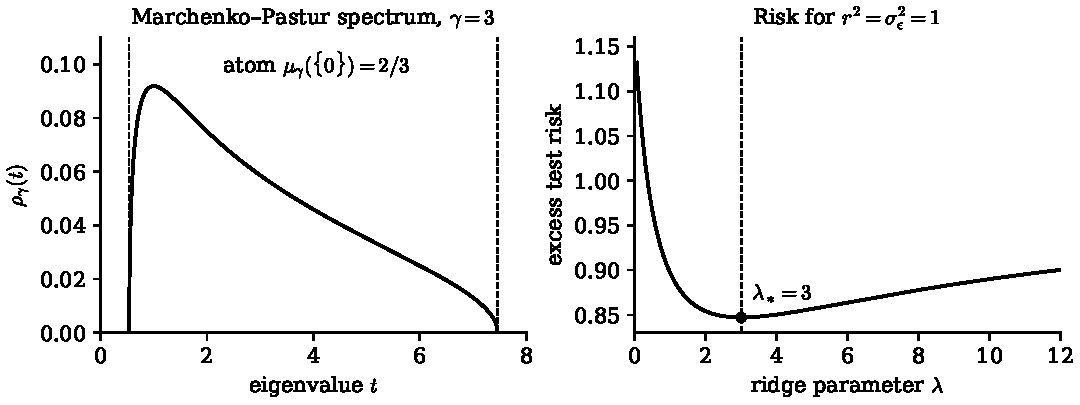
\includegraphics[width=\textwidth]{figures/ridge_gamma3.pdf}
    \caption{
        High-dimensional linear regression at aspect ratio
        \(\gamma=d/n=3\).
        Left: the continuous part of the Marchenko--Pastur spectrum;
        an additional atom of weight \(2/3\) sits at zero.
        Right: the asymptotic excess prediction risk of ridge
        regression for \(r^2=\sigma_\epsilon^2=1\).
        The minimum occurs at
        \(\lambda_*=\gamma\sigma_\epsilon^2/r^2=3\).
    }
    \label{fig:ridge_gamma3}
\end{figure}


% ============================================================
\section{Summary: the recurring idea}
% ============================================================

These examples illustrate the same general principle:
large systems are often controlled not by the raw sizes
individually, but by a small number of \emph{dimensionless ratios}.

\begin{equation}
\boxed{
\begin{array}{ccl}
\text{deep linear network}
&:&
\xi=L/N,
\\[1mm]
\text{ResNet}
&:&
L s_L^2
\quad
\text{(iid case)},
\\[1mm]
\text{high-dimensional regression}
&:&
\gamma=d/n.
\end{array}
}
\end{equation}

The goal of scaling theory is therefore to identify:

\begin{enumerate}
    \item the correct macroscopic variables;
    \item the dimensionless combinations that remain finite;
    \item the corresponding limiting dynamics;
    \item the scaling of hyperparameters required to obtain a
    non-trivial limit.
\end{enumerate}

This is the basic philosophy behind studying neural networks
through large-\(N\), large-\(L\), large-data, and large-training-time
limits.
